% Define functions for connecting a question and answer to each other.
\newcommand{\refQ}[1]{\vspace{1em} \hfill (\hyperref[#1]{Question on page \pageref{#1}})}
\newcommand{\refA}[1]{\vspace{1em} \hfill (\hyperref[#1]{Answer on page \pageref{#1}})}

\lesson{}{Maths}

% \subsection{Probability}

% \subsubsection{Definitions}

% \begin{definition}[outcome space]
%     a set of all possible outcomes of some kind
%     \\~\\
%     the outcome space is often referred to as $\Omega$
% \end{definition}
% \begin{definition}[event]
%     a subset of the outcome space
%     \\~\\
%     In general, event $i$ can be referred to as $E_i$. However, events are often referred to as $A$, $B$, and so on.
% \end{definition}
% \begin{definition}[probability]
%     a function that maps events or subsets to a number between 0 and 1
%     \\~\\
%     probability is often referred to as $P[\cdot]$
% \end{definition}

% \begin{example}[A fair six-sided dice]
%     The outcome space, $\Omega$, would be the set of all possible outcomes, $\{1,2,3,4,5,6\}$. A possible event would be rolling an even number, $E_{\text{even}}$, which is a subset of the outcome space, $\{2,4,6\}$. Finally, a probability is the function that maps an event to a number between 0 and 1. For even numbers, the probability is $P[E_{\text{even}}] = 0.5$. Hopefully, the 0.5 probability of rolling an even number from a fair six-sided dice is no surprise. But the probability function depends a number of factor, and can be fairly involved. How one defines and determines the probability for a given event will become clear soon. 
% \end{example}

% \begin{definition}[union]
%     a union is the union of two subsets
%     \\~\\
%     union is often referred to as $\cup$
% \end{definition}

% \begin{definition}[intersection]
%     an intersection is the intersection of two subsets
%     \\~\\
%     intersection is often referred to as $\cap$
% \end{definition}

% \begin{definition}[complement]
%     the complement of an event is the subset of outcomes of the event not happening
%     \\~\\
%     complement of event $A$ is often referred to as $A^c$
% \end{definition}



% \subsubsection{Expectations}

% \subsection{Statistics}


\newpage
\subsection{Linear Algebra}
% \label{sub_sec:linearAlg}

\subsubsection{Definitions}

\begin{definition}[Null space]
The null space of a matrix $\mathbf{A}_{m \times n}$, $\mathrm{Null}(\mathbf{A})$,  is the set of vectors whose multiplication with $\mathbf{A}$ results in the zero vector.

\begin{equation}
    \{ \mathbf{x} \in \mathbb{R}^n | \mathbf{A} \mathbf{x} = \mathbf{0} \}
\end{equation}

\end{definition}

\begin{definition}[Column space]
The column space of a matrix $\mathbf{A}_{m \times n}$, $\mathrm{Col}(\mathbf{A})$,  is the set of all possible vectors $\mathbf{b}$ that result from multiplying  $\mathbf{A}$ by any vector $\mathbf{x} \in \mathbb{R}^n$.

\begin{equation}
    \{ \mathbf{b} \in \mathbb{R}^m | \mathbf{A} \mathbf{x} = \mathbf{b} \}
\end{equation}

\end{definition}

\newpage
\subsection{Calculus}
\label{sub_sec:calc}
\textit{Credit: Reece Huff}
\subsubsection{Fundamentals}
\subsubsection{Einstein summation notation}

Einstein summation notation is a shorthand way of writing mathematical expressions that involve repeated summations or products over indices. It is widely used in fields such as physics and engineering to write complex equations in a more concise and elegant form.

In Einstein summation notation, repeated indices are automatically summed over, unless they appear once in a subscript and once in a superscript. This convention is known as the Einstein summation convention. The indices are typically Greek letters for time indices, and Latin letters for spatial indices.

In this notation, scalars, vectors, and matrices are represented as follows:
\begin{itemize}
    \item Scalars are represented by a single symbol, such as $a$ or $f$.
    \item Vectors are represented by lowercase Latin letters with indices, such as $v_i$ or $u_j$. The indices can take on values of 1, 2, ..., $n$, where $n$ is the dimension of the vector.
    \item Matrices are represented by uppercase Latin letters with two indices, such as $A_{ij}$ or $B_{kl}$. The first index refers to the row number and the second index refers to the column number.
\end{itemize}

Using this notation, we can write linear algebra equations more compactly and with less clutter. For example, the dot product of two vectors $\mathbf{u}$ and $\mathbf{v}$ can be written as:

\begin{align}
\mathbf{u} \cdot \mathbf{v} = u_i v_i
\end{align}

Similarly, the matrix-vector product $\mathbf{y} = A \mathbf{x}$ can be written as:

\begin{align}
y_i &= A_{ij} x_j
\end{align}

Einstein summation notation can also be used for expressing more complex operations such as matrix multiplication, transpose, and inverse.

\paragraph{Kronecker Delta:}
\begin{align}
    \delta_{ij} = \mathbf{e}_i \cdot \mathbf{e}_j = 
    \begin{cases}
        1 & i=j \\
        0 & i\neq j
    \end{cases}
\end{align}

\paragraph{Dot Product:}
\begin{align}
\mathbf{u} \cdot \mathbf{v} = (u_i \mathbf{e}_i) \cdot (v_j \mathbf{e}_j) = u_i v_j \mathbf{e}_i \cdot \mathbf{e}_j = u_i v_j \delta_{ij} = u_i v_i
\end{align}

\paragraph{Alternating (Epsilon or Levi-Civita) Symbol:}
\begin{align}
    \epsilon_{ijk} &= \begin{cases}
    1 & i,j,k \text{ is an even permutation}\\
    0 & i=j \text{ or } i=k \text{ or } j=k\\
    -1 & i,j,k \text{ is an odd permutation}
\end{cases}
\end{align}

\paragraph{Cross Product:}
\begin{align}
    u\times v &= \epsilon_{ijk} u_j v_k e_i 
    \\
    (u\times v)i &= \epsilon{ijk} u_j v_k
\end{align}

\paragraph{Relationship between the Alternating Symbol and the Kronecker Delta:}
\begin{align}
\epsilon_{ijk} \epsilon_{ilm} &= \delta_{jl} \delta_{km} - \delta_{jm} \delta_{kl}
\end{align}

\paragraph{Tensor (Dyadic) Product:}
\begin{align}
(a\otimes b)u &= a(b\cdot u)
\\
(a\otimes b)_{ij} &= a_i b_j
\\
(a\otimes b)(a\otimes b) &= a(b\cdot a)\otimes b
\\
(a\otimes b) &= (a_i e_i)\otimes (b_j e_j) = a_i b_j e_i\times e_j
\\
I &= \delta_{ij} e_i\otimes e_j = e_i\otimes e_i
\end{align}

\paragraph{Gradient of Scalar Field:} 
The gradient of a scalar field is a vector that points in the direction of the greatest increase of the function at a given point. It is denoted by the symbol $\nabla$.

In Cartesian coordinates, the gradient of a scalar function $f(x,y,z)$ is defined as:

\begin{align}
\nabla f &= \frac{\partial f}{\partial x} \mathbf{i} + \frac{\partial f}{\partial y} \mathbf{j} + \frac{\partial f}{\partial z} \mathbf{k},
\end{align}

where $\mathbf{i}, \mathbf{j},$ and $\mathbf{k}$ are the unit vectors along the $x,y,$ and $z$ axes, respectively.

More generally, the gradient of a scalar field $f(\mathbf{x})$ in $n$-dimensional space can be written as:

\begin{align}
\nabla f &= \frac{\partial f}{\partial x_1} \mathbf{e_1} + \frac{\partial f}{\partial x_2} \mathbf{e_2} + \cdots + \frac{\partial f}{\partial x_n} \mathbf{e_n},
\end{align}

where $\mathbf{e_1}, \mathbf{e_2}, \dots, \mathbf{e_n}$ are the unit vectors along the $n$ coordinate axes.

By convention, if we wish to represent the gradient of a scalar function $f(\mathbf{x})$ as a vector in direct notation, we write it as a column vector:

\begin{align}
\nabla f &= \begin{bmatrix}
\frac{\partial f}{\partial x_1} 
\\
\frac{\partial f}{\partial x_2} 
\\
\vdots 
\\
\frac{\partial f}{\partial x_n}
\end{bmatrix}
\end{align}

This makes sense because the gradient is a vector quantity, and vectors are typically represented as column vectors.

\begin{example}
    Let's consider the scalar function $f(\mathbf{x}) = \mathbf{x}^T A \mathbf{x}$, where $A \in \mathbb{R}^{n \times n}$. The gradient of this function with respect to $\mathbf{x}$ is:
    
    \begin{align}
    \nabla_{\mathbf{x}} f &= \frac{\partial f}{\partial x_i} e_i \\
    &= \frac{\partial}{\partial x_i} (x_j a_{jk} x_k) e_i \\
    &= (2 a_{ij} x_j) e_i + (a_{jk} x_k) \frac{\partial x_j}{\partial x_i} e_i \\
    &= (A + A^T)_{ij} x_j e_i,
    \end{align}
    
    where we used the product rule for partial differentiation and the fact that $A$ is symmetric. The expression $(A + A^T)_{ij}$ represents the $(i,j)$-th entry of the matrix $A + A^T$.
\end{example}

\paragraph{Gradient of Vector Field:}
\begin{align}
\nabla v &= \frac{\partial v_i}{\partial x_j} e_i\otimes e_j
\end{align}

\newpage
\subsection{Differential Equations}
% \label{sub_sec:diffeq}


\subsubsection{Parabolic Partial Differential Equations}

Parabolic partial differential equations (PDEs) play a fundamental role in modeling various phenomena, ranging \textit{from black holes to Black-Scholes}. More specifically, the form of parabolic PDEs elegantly captures the dynamics of a large range processes such as heat and chemical diffusion, Schrödinger's equation, and option pricing in financial mathematics. One of the most commonly used numerical methods for solving such equations is the finite difference method (FDM). FDM is a simple, efficient, and robust technique that discretizes the PDE on a grid and approximates the derivatives using finite differences \cite{leveque_fdm}. This method has been extensively studied and applied in various fields of science and engineering for over a century. In this section of the dissertation, I discuss the theoretical foundations and practical implementation of FDM for parabolic PDEs.

\begin{equation}\label{eq:heat}
    \underbrace{u_t}_{\textit{time differential}} - \underbrace{\nabla_x \cdot (\kappa \nabla_x u))}_{\textit{diffusion of quantity $u$}} = \underbrace{f_m}_{\textit{source terms}}
\end{equation}

The general form of the classic heat equation is shown in \Cref{eq:heat} where $u$ models temperature or chemical concentration at a given point in space and time, $\kappa$ is the heat capacity or diffusion coefficient (possibly temporally and/or spatially dependent), and $f_m, \ \forall m = 1, ..., M$ nodes are the source term (also possibly temporally and/or spatially dependent). To solve the heat equation numerically, it is necessary to specify both initial conditions and boundary conditions. The initial conditions specify the temperature distribution within the domain at time zero, while the boundary conditions specify the behavior of the solution at the boundaries of the domain. Dirichlet boundary conditions prescribe the temperature on the boundary, while Neumann boundary conditions prescribe the flux through the boundary. These boundary conditions are required because they provide the necessary information to obtain a unique solution to the heat equation. Without boundary conditions, the solution would not be well-defined, and there would be an infinite number of possible solutions that satisfy the PDE. Therefore, the appropriate choice of boundary conditions is crucial for obtaining physically meaningful solutions to the heat equation.

Concretely, a well-defined parabolic PDE consists of: 

\begin{enumerate}
    \item PDE: \quad\quad\quad\quad\quad\quad\quad $u_t - \nabla_x \cdot (\kappa \nabla_x u) = f, \quad x\in \Omega, \quad t>0$ 
    \item Initial condition: \quad\quad $u(x, t=0) = \eta(x), \quad x \in \Omega$
    \item Boundary conditions: $\Gamma = \partial \Omega$ 
    \begin{itemize}
        \item Dirichlet boundary condition: $u = u_D$ on $\Gamma \times(0, T)$ which directly prescribes the temperature or chemical concentration. 
        \item Neumann boundary condition:   $(\kappa \nabla_x u)\cdot \boldsymbol{n} = g_M$ on $\Gamma \times(0, T)$ which prescribes the heat or diffusion flux across the boundary. 
    \end{itemize}
\end{enumerate}

\subsubsection{Finite Difference Grid}

For simple geometries, the finite difference grid provides a straight-forward approach to discretizing the domain into a finite number of points or nodes. Each node represents a discrete location where the solution is evaluated, and the solution at each node is approximated using a finite difference approximation (example in \Cref{fig:fdgrid}). 

\FloatBarrier
\begin{figure}[ht]
   \centering
   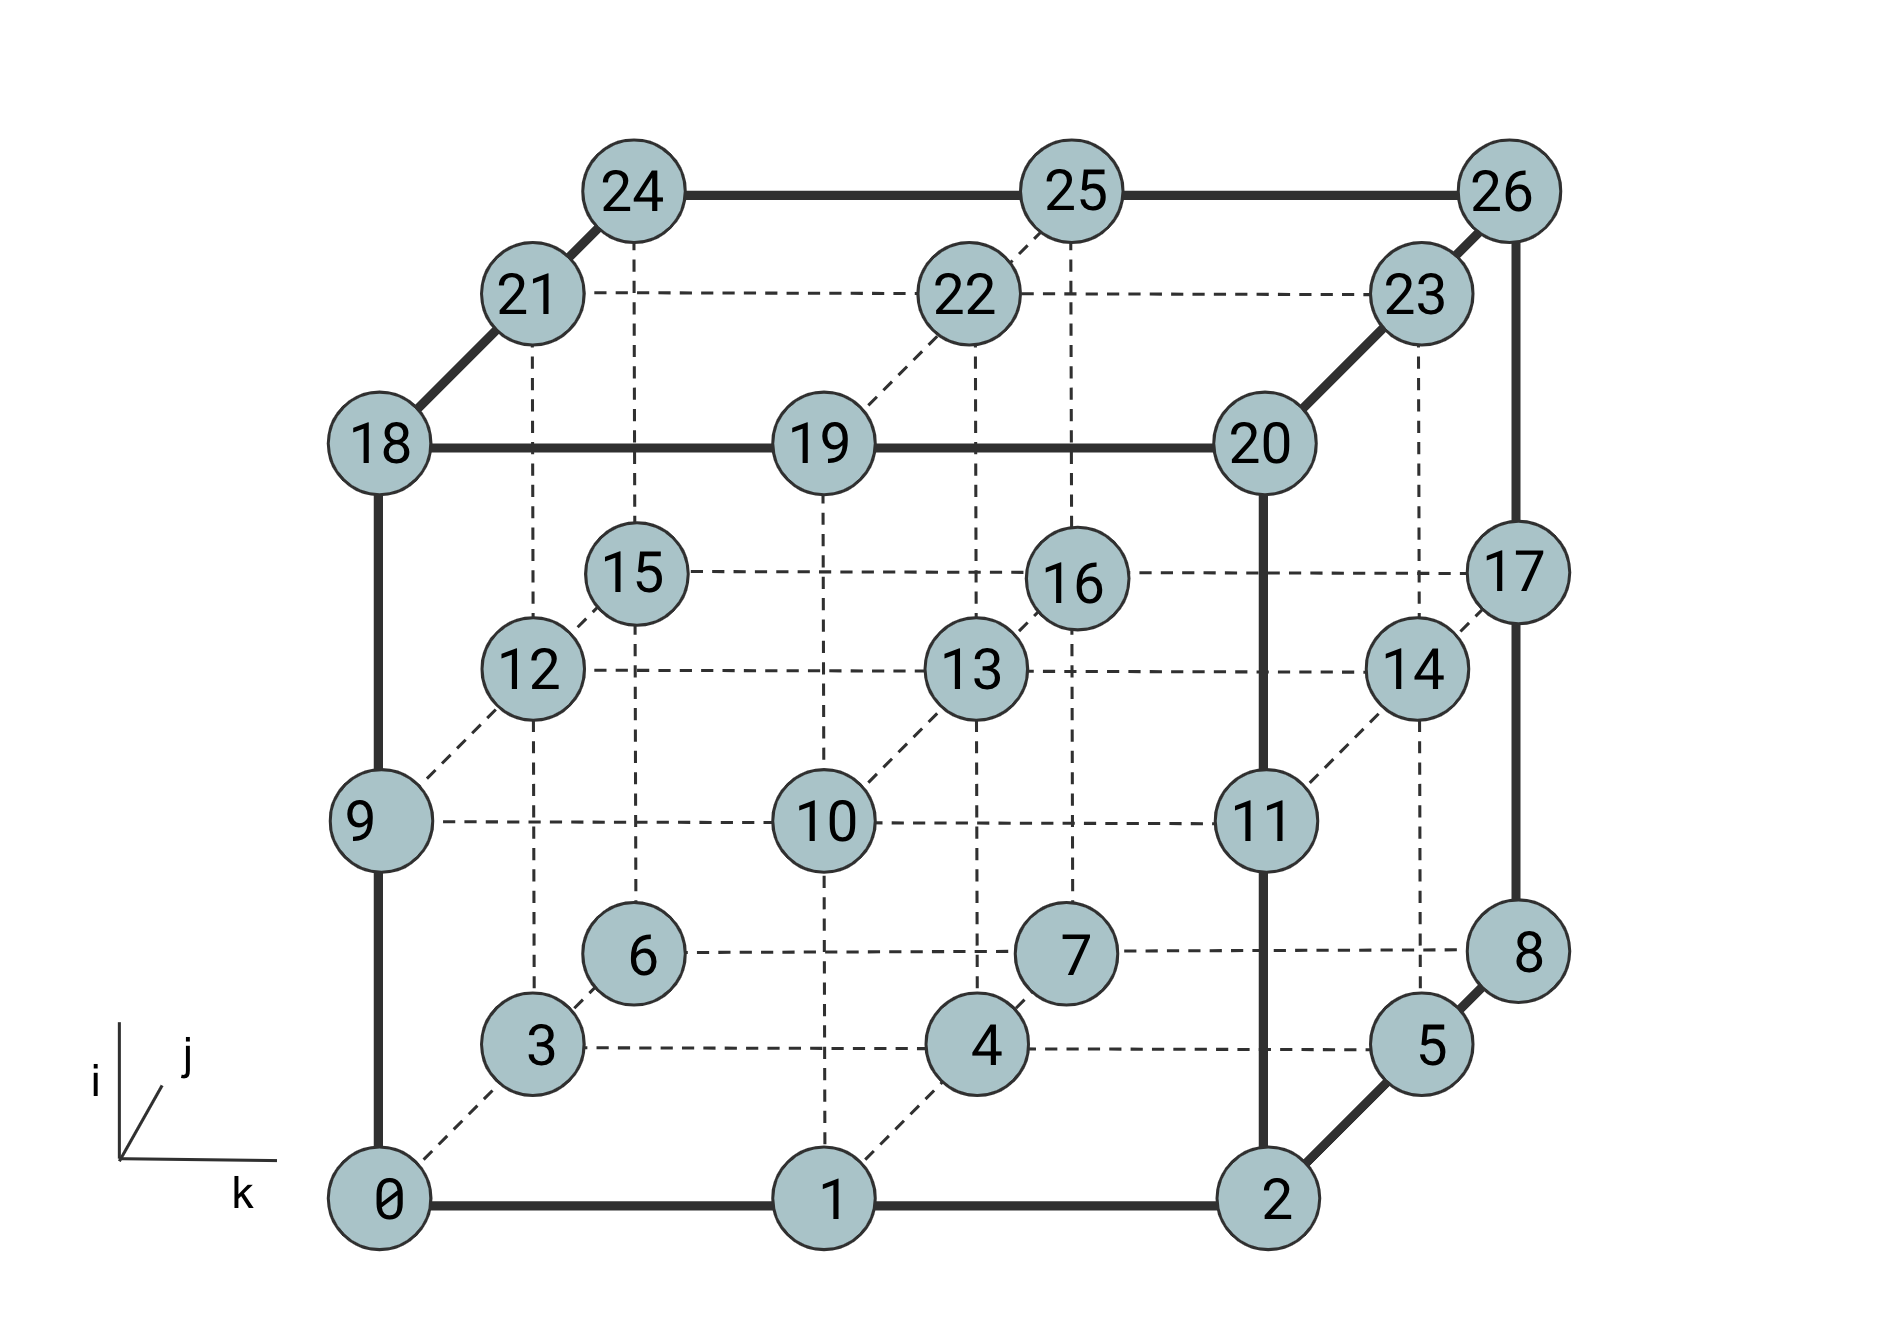
\includegraphics[width=0.85\textwidth]{figures/fdgrid.png}
   \caption{An example 3D finite difference grid where each node is equally spaced from neighboring nodes by some amount $\Delta x = \frac{L}{M-1}$, where $L$ is the length of the domain across a single axis, and $M$ are the total number of nodes along that same axis. }
   \label{fig:fdgrid}
\end{figure}
\FloatBarrier

The accuracy of the FDM depends on the \textit{size of the grid} and \textit{the order of the finite difference approximation} used. In this way, the spatial domain of the PDE is transformed into a discrete set of equations that can be solved numerically using linear algebra techniques. The choice of grid size and finite difference approximation is critical in achieving a stable and accurate numerical solution.

\subsubsection{Finite Difference Methods}
\noindent\textbf{Forward Difference in Time, Centered in Space (FTCS)}

We seek to find an approximate solution $U_m^n \approx u(x_m, t_n)$ by approximating the diffusion term in \Cref{eq:heat} which will enable us to ``march forward in time", computing $U_m^{n+1} \ \forall \ m = 1, \dots, M$ as a function of $U_m^n$ at the previous time step. 

FTCS seeks to find an approximate solution $U_m^n \approx u(x_m, t_n)$ by spatially discretizing the domain into a finite number of equally spaced grid points and approximates the spatial derivative at each point using a centered difference formula. The temporal derivative is approximated using a forward difference formula, and the solution at each grid point is updated at each time step based on the values at its neighboring points in space and the previous time step.

To obtain the FTCS approximation for $x \in \mathcal{R}^1$, we first consider a second-order center-difference approximation \cite{leveque_fdm} of the Laplacian of the flux:


\begin{equation}
    \nabla_x \cdot \boldsymbol{q} = \frac{\partial q}{\partial x} \approx \frac{q(x_1 + h/2) - q(x_1 - h/2)}{h}
\end{equation}

where $\boldsymbol{q} = \kappa \nabla_x u$ and $h = \Delta x$. Assuming $\kappa$ is constant in space, each partial flux can be further approximated by applying a successive first-order one-sided approximation: 

\begin{align}
    q\big(x + h/2\big) &\approx \kappa \frac{u(x+h) - u(x)}{h} \\
    q\big(x - h/2\big) &\approx \kappa \frac{u(x) - u(x-h)}{h}
\end{align}

yielding the centered-in-space approximation:

\begin{equation}
    \frac{\partial}{\partial x}\big(\kappa \frac{\partial u}{\partial x}\big) = \kappa u_{xx} \approx \kappa \frac{u(x-h) - 2u(x) + u(x+h)}{h^2}. 
\end{equation}


Finally, the time derivative on the left-hand side of \Cref{eq:heat} is approximated using a first-order one-sided approximation

\begin{equation}\label{eq:ftcs}
    U_{m}^{n+1} = U_{m}^{n} + \frac{k \kappa}{h^2}\big(U_{m-1}^{n} - 2 U_{m}^{n} + U_{m+1}^{n}\big) + \frac{k}{h^2}f(U_m^n, t_n) 
\end{equation}

where $k = \Delta t$. This method is more commonly referred to as the \textit{Forward Euler} time stepping scheme. The FTCS method is considered to be a first-order accurate in time, and second-order accurate in space. Since the right-hand side of \Cref{eq:ftcs} is only dependent on $U_m^{n}$ at the previous time step (all of which are known), this scheme is considered to be in an \textit{explicit method} since $U_m^{n+1}$ can be explicitly computed. 

\vspace{0.5cm}
\noindent\textbf{Trapezoidal Method}

Like the FTCS method, the trapezoidal method also employs a second-order center-difference approximation for the spatial discretization of the diffusion term in \Cref{eq:heat}. However, rather than using an exclusive forward difference scheme, the trapezoidal method employs a weighted average of backward and forward differences in time parameterized by $\phi \in [0, 1]$: 

\begin{equation}
\begin{aligned}
U_m^{n+1} = & \quad U_m^n \\
&+ \phi \frac{k}{h^2} \bigg(\kappa (U_{m-1}^{n} - 2U_{m}^{n} + U_{m+1}^{n}) + f(U_{m}^{n}, t_n) \bigg)\\
&+ (1-\phi) \frac{k}{h^2} \bigg(\kappa\underbrace{(U_{m-1}^{n+1} - 2U_{m}^{n+1} + U_{m+1}^{n+1}) + f(U_{m}^{n+1}, t_n)}_{U_m^{n+1} \textit{ is unknown}}\bigg).
\end{aligned}
\end{equation}

When $\phi=1/2$, the trapezoidal method reduces to the \textit{Crank-Nicholson} method. The trapezoidal/Crank-Nicholson method is considered to be a second-order accurate in time, and second-order accurate in space. Since the right-hand side of \Cref{eq:ftcs} is only dependent on both $U_m^{n}$ at the previous time step (all of which are known) and $U_m^{n+1}$ at the next time step (all of which are unknown), this scheme is considered to be in an \textit{implicit method} since $U_m^{n+1}$ must be implicitly computed. 

\vspace{0.5cm}
\begin{tcolorbox}[colback=gray!5!white,colframe=gray!75!black]
\noindent \textit{Example: Crank-Nicholson for linear PDEs}
\vspace{0.25cm}

Consider the simple parabolic PDE: 

\begin{equation}\label{eq:heat_simple}
    u_t = u_{xx}. 
\end{equation}

The Crank-Nicholson method discretizing \Cref{eq:heat_simple} yields: 

\begin{equation}
    U_m^{n+1} = U_m^{n} + \frac{k}{2h^2} \bigg(U_{m-1}^{n} - 2U_{m}^{n} + U_{m+1}^n + U_{m-1}^{n+1} - 2U_{m}^{n+1} + U_{m+1}^{n+1}\bigg). 
\end{equation}

In the case in which the PDE is linear, we can move all terms containing the unknown solutions $U_m^{n+1}$ at the text time step to the left-hand side and leave all of the known solutions $U_m^n$ at the previous time step on the right-hand side: 

\begin{equation}\label{eq:cranknic}
    -\frac{k}{2h^2}U_{m-1}^{n+1} + (1+2\frac{k}{2h^2})U_{m}^{n+1} - \frac{k}{2h^2}U_{m+1}^{n+1} = \underbrace{\frac{k}{2h^2}U_{m-1}^{n} + (1-2\frac{k}{2h^2})U_{m}^{n} - \frac{k}{2h^2}U_{m+1}^{n}}_{\textit{known }\boldsymbol{b}}.
\end{equation}

Our known solutions at the previous and next time steps can be organized as vectors $\boldsymbol{U}_{m}^{n}$, $\boldsymbol{U}_{m}^{n+1} \in \mathcal{R}^{m_{nodes}}$ respectively. This means we can re-write the left-hand side of \Cref{eq:cranknic} as system of $M$ equations, and the right-hand side as a single column vector: 

\begin{equation}\label{eq:cranknic_mol}
    \underbrace{
    \begin{bmatrix}
        (1 + 2\frac{k}{2h^2}) & - \frac{k}{2h^2}      &          0       & \dots            &  &  & 0\\
        - \frac{k}{2h^2}      & (1 + 2\frac{k}{2h^2}) & - \frac{k}{2h^2} & \dots            &   &  & \vdots\\
        0                     & \ddots                & \ddots           & \ddots           &  &  &  \\
        \vdots                &                       &                  & - \frac{k}{2h^2} & (1 + 2\frac{k}{2h^2}) & - \frac{k}{2h^2}     \\
        0                     &                       &       \dots       &                  & - \frac{k}{2h^2}      & (1 + 2\frac{k}{2h^2})\\
    \end{bmatrix}
    }_{\boldsymbol{A}}
    \underbrace{
    \begin{bmatrix}
        U_{1}^{n+1} \\
        U_{2}^{n+1} \\
        \vdots \\
        U_{M-1}^{n+1} \\
        U_{M}^{n+1} \\
    \end{bmatrix}
    }_{\boldsymbol{x}}
    = 
    \boldsymbol{b}
\end{equation}

where 

\begin{equation*}
    \boldsymbol{b} = 
    \begin{bmatrix}
        \frac{k}{2h^2}\big(g_0(t_{n}) + g_0(t_{n+1})\big) + (1 - \frac{k}{2h^2})U_1^n + \frac{k}{2h^2}U_2^n \\
        \frac{k}{2h^2}U_1^n + (1-2\frac{k}{2h^2})U_2^n + \frac{k}{2h^2}U_3^n \\
        \vdots \\
        \frac{k}{2h^2} U_{M-2}^n + (1-2\frac{k}{2h^2})U_{M-1}^n + \frac{k}{2h^2}U_M^n \\
        \frac{k}{2h^2}U_{M-1}^n + (1-2\frac{k}{2h^2}) + \frac{k}{2h^2}\big(g_1(t_{n}) + g_1(t_{n+1})\big) \\
    \end{bmatrix}
\end{equation*}

which reduces to solving $\boldsymbol{Ax} = \boldsymbol{b}$. Since $\boldsymbol{A}$ is tri-diagonal, this problem can be solved as efficiently as an explicit method. 
\end{tcolorbox}

% The trapezoidal method is a finite difference method that employs a combination of backward and forward differences to approximate the solution to a differential equation at discrete time steps. The trapezoidal method is a second-order accurate scheme that is unconditionally stable and can handle stiff equations. It is commonly used in solving the heat equation in one dimension using the forward in time, centered in space (FTCS) numerical scheme. In this approach, the spatial derivative is approximated using a centered difference, while the temporal derivative is approximated using a forward difference. 

\subsubsection{Analysis of Numerical Methods}
\vspace{0.25cm}
\noindent\textit{Local Truncation Error and Order of Accuracy}
\vspace{0.25cm}

Numerical methods provide approximate solutions for ODEs/PDEs, and the accuracy of the solutions are dependent on the time discretization $k = \Delta t$ and spatial discretization $h = \Delta x$. After taking a single time step, some amount of error is introduced to the solution, also referred to as the local truncation error (LTE). This provides a method for analyzing the order of accuracy of a numerical method and how the quickly the error decreases as $h, \ k \rightarrow 0$. The LTE for the simple ODE $u_t = \lambda u + f(t)$ with an initial value $u(0) = u_0$ for the Backward Euler time discretization method is: 

\begin{equation}\label{eq:trunc_err}
    \tau_n = \frac{u(t_n) - u(t_{n-1})}{k} - \lambda u(t_n) - f(t_n), \quad \forall n = 1, ..., N
\end{equation}

 Order of accuracy is a measure of how well a finite difference method approximates a solution to a differential equation and describes how quickly the error between the approximate solution and the true solution decreases as $k, \ h \rightarrow 0$. Intuitively, a method will converge to the true solution at rate proportional to the order of accuracy. For example, a method with second order of accuracy in space will have an error that decreases proportional to the square of the grid spacing. Although we \textit{expect} the approximate solution to approach the true solution such that the error of the method $||\tau(x,t)|| \rightarrow 0$, for convergence to the true solution to occur, the temporal and spatial discretization must satisfy a the two properties: consistency and stability. 

\vspace{0.25cm}
 \noindent\textit{Consistency}
 \vspace{0.25cm}
 
As both $h, \ k \rightarrow 0$, the we \textit{expect} the approximate solution to approach the true solution such that the LTE of the method $||\boldsymbol{\tau}|| \rightarrow 0$. If this is indeed true, the discretization method is said to be \textit{consistent}, meaning that the discrete equation approximates the same process as the underlying PDE as the temporal and spatial grids become finer at a rate that is at least as fast as $h, \ k \rightarrow 0$.

More concretely, \textit{consistency} requires: 

\begin{equation}
    ||\boldsymbol{\tau}||_{\infty} = \max_{n = 1, \dots, N} \ |\tau_n| \ \rightarrow 0 \text{ as } \Delta t \rightarrow 0. 
\end{equation}

In the \textit{LTE and order of accuracy for the Crank-Nicolson Method} example, the LTE is shown to be $\mathcal{O}(k^2+h^2)$. A method is said to be \textit{consistent} since the global order of accuracy will agree with the order of the LTE: 

\begin{equation}
    U_m^n - u(X,T) = \mathcal{O}(k^2 + h^2). 
\end{equation}
 
 To determine whether a method is consistent, we need to analyze LTE. The following are two examples for deriving the LTE and order of accuracy for the \textit{Forward in Time, Centered in Space} and \textit{Crank-Nicolson} methods, and how the error corresponds to $k, \ h$. 


% As both $h, \ k \rightarrow 0$, the we \textit{expect} the approximate solution to approach the true solution such that the error of the method $||\tau(x,t)|| \rightarrow 0$.



% Numerical methods provide approximate solutions for the PDE, and the accuracy of the solutions is dependent on the time discretization $k = \Delta t$ and spatial discretization $h = \Delta x$. As both $h, \ k \rightarrow 0$, the we \textit{expect} the approximate solution to approach the true solution such that the error of the method $||\tau(x,t)|| \rightarrow 0$. If true, the method is said to be \textit{consistent}. Typically $||\tau(x,t)^h|| = \mathcal{O}(h^p)$ for some integer $p > 0$, and then the method is certainly consistent \cite{leveque_fdm}. 

% This also indicates that after taking a single time step, some amount of error is introduced to the solution, also referred to as the local truncation error (LTE). Once we compute the LTE of the method, the stability of the method can be computed by showing that the global error can be bounded in terms of the LTE. 

% 


\vspace{0.5cm}
\begin{tcolorbox}[colback=gray!5!white,colframe=gray!75!black]
\noindent\textit{Example: LTE and order of accuracy for FTCS method}

Consider the simple parabolic PDE $u_t = u_{xx}$. The resulting error for a chosen time step $k$ and for a chosen spatial step $h$ for \Cref{eq:ftcs} is defined as:

% \begin{equation}\label{eq:ftcs}
%     U_{m}^{n+1} = U_{m}^{n} + \frac{\kappa}{h^2}\big(U_{m-1}^{n} - 2 U_{m}^{n} + U_{m+1}^{n}\big) + \frac{k}{h^2}f(u(x, t), t_n) 
% \end{equation}

\begin{equation}
    \tau(x, t) = \frac{U_{m}^{n+1} - U_{m}^{n}}{k} - \frac{\kappa}{h^2}\big(U_{m-1}^{n} - 2 U_{m}^{n} + U_{m+1}^{n}\big). 
\end{equation}

To obtain the LTE, insert the true solution: 

\begin{equation}\label{eq:ftcs_lte}
    \tau(x, t) = \frac{u(x, t+k) - u(x, t)}{k} - \frac{\kappa}{h^2}\big(u(x-h, t) - 2 u(x, t) + u(x+h, t)\big)
\end{equation}

For the first term on the right-hand side, we care about the error relative to $k$, and for the second term we care about the error relative to $h$. If we make the assumption that $u$ is smooth, we can expand each term around $k, \ h$ respectively: 

Assuming that $u$ is sufficiently smooth and differentiable, each $u$ term containing increment in $k$ and $h$ can be expanded in a Taylor series: 

\begin{align}%\label{eq:ftcs_expand}
    u(x, t+k) &= u + k u_t + \frac{1}{2} k^2 u_{tt} + \frac{1}{6} k^3 u_{ttt} + \mathcal{O}(t^4) \label{eq:ftcs_expand1}\\
    u(x-h, t) &= u - h u_x + \frac{1}{2} h^2 u_{xx} - \frac{1}{6} h^3 u_{xxx} + \mathcal{O}(h^4) \label{eq:ftcs_expand2}\\
    u(x+h, t) &= u + h u_x + \frac{1}{2} h^2 u_{xx} + \frac{1}{6} h^3 u_{xxx} + \mathcal{O}(h^4)\label{eq:ftcs_expand3}. 
\end{align}

Inserting each Taylor series expansion from \Cref{eq:ftcs_expand1}, \Cref{eq:ftcs_expand2}, and \Cref{eq:ftcs_expand3} into \Cref{eq:ftcs_lte} yields: 

\begin{equation}
    \tau(x, t) = \bigg(\underbrace{u_t}_{= \ u_{xx}} + \underbrace{\frac{1}{2} k u_{tt}}_{= \ u_{txx} = \ u_{xxxx}} + \ \mathcal{O}(k^2) \bigg) - (u_{xx} + \frac{1}{12}h^2 u_{xxxx} + \mathcal{O}(h^3) \bigg) 
\end{equation}

Recall that $u_t = u_{xx}$ and $u_{tt} = u_{xxxx}$ allowing for additional terms to simplify: 

\begin{equation*}
    \tau(x,t) = \big(\frac{1}{2}k - \frac{1}{12}h^2\big) u_{xxxx} = \mathcal{O}(k + h^2). 
\end{equation*}

This derivation shows that the error for the FTCS method is expected to increase linearly with $k$ and to increase with the power of two with $h$. This is more commonly stated to be \textit{first-order accurate in time, and second-order accurate in space}. 

\end{tcolorbox}
\vspace{0.5cm}

\vspace{0.5cm}
\begin{tcolorbox}[colback=gray!5!white,colframe=gray!75!black]
\noindent\textit{Example: LTE and order of accuracy for the Crank-Nicolson method}

Once again, consider the simple parabolic PDE $u_t = u_{xx}$. The resulting error for a chosen time step $k$ and for a chosen spatial step $h$ is defined as: 

\begin{equation}
    \tau(x,t) = \frac{U_m^{n+1} - U_m^{n}}{k} + \frac{1}{2h^2} \bigg(U_{m-1}^{n} - 2U_{m}^{n} + U_{m+1}^n + U_{m-1}^{n+1} - 2U_{m}^{n+1} + U_{m+1}^{n+1}\bigg). 
\end{equation}

To obtain the LTE, insert the true solution: 
\begin{equation}
    \begin{aligned}
        \tau(x,t) \ = 
        \ & \ \frac{u(x,t+k) - u(x,t)}{k} \\ 
        \ & + \frac{1}{2h^2} \bigg(u(x-h, t) -2u(x,t) + u(x+h, t) \\
        \ & \quad\quad\quad \ \  + \ u(x-h, t+k) - 2u(x, t+k) + u(x+h, t+k) \bigg). 
    \end{aligned} \label{eq:cranknic_err}
\end{equation}

Once again assuming the true solution $u$ is sufficiently smooth and differentiable, the Taylor series expansion for $u(x,t+k)$, $u(x-h,t)$ and $u(x+h,t)$ can be recycled from \Cref{eq:ftcs_expand1}, \Cref{eq:ftcs_expand2}, \Cref{eq:ftcs_expand3}. For $u(x-h, t+k)$ and $u(x+h, t+k)$, a multi-variable Taylor series expansion is required:

\begin{align}
    u(x-h, t+k) &= u - h u_x + k u_t + \frac{1}{2}h^2u_{xx} - hk u_{tx} + \frac{1}{2}k^2u_{tt} + \mathcal{O}(h^3, k^3, h^2k, hk^2) \label{eq:cranknic_expand1}\\
    u(x+h, t+k) &= u + h u_x + k u_t + \frac{1}{2}h^2u_{xx} + hk u_{tx} + \frac{1}{2}k^2u_{tt} + \mathcal{O}(h^3, k^3, h^2k, hk^2) \label{eq:cranknic_expand2}. 
\end{align}

Inserting each Taylor series expansion from Equations \ref{eq:ftcs_expand1}-\ref{eq:ftcs_expand3} and Equations \ref{eq:cranknic_expand1}-\ref{eq:cranknic_expand2} into \Cref{eq:cranknic_err} and a lot of tedious cancellation of terms yields: 

\begin{equation}
    \tau(x,t) = \mathcal{O}(k^2, h^2). 
\end{equation}

This derivation shows that the error for the Crank-Nicolson method is expected to increase with the power of two with $k$ and to increase with the power of two with $h$. This is more commonly stated to be \textit{second-order accurate in time, and second-order accurate in space}. 

\end{tcolorbox}

\newpage 



\vspace{0.5cm}
\noindent\textit{Stability}

Small variations in the initial and boundary conditions may cause sensitive numerical methods to be unstable. These small LTEs may cause the approximate solution to diverge from the true solution over time since each error may compound on itself. For time-dependent ODEs, the concept of \textit{absolute stability} allows us to analyze terms that recursively amplify or dampen a solution after a time step. The stability theory for time-dependent PDEs can be related to the stability theory for time-dependent ODEs through the method of lines (MOL) discretization of the PDE (see \Cref{fig:mol}). The MOL approach first discretizes in space alone, resulting in a system of ODEs that can be solved using methods for ODEs. This system of ODEs is known as a semi-discrete method since it is discretized in space but not yet in time.

\begin{figure}[htbp] % specify figure placement
    \centering % center the figure
    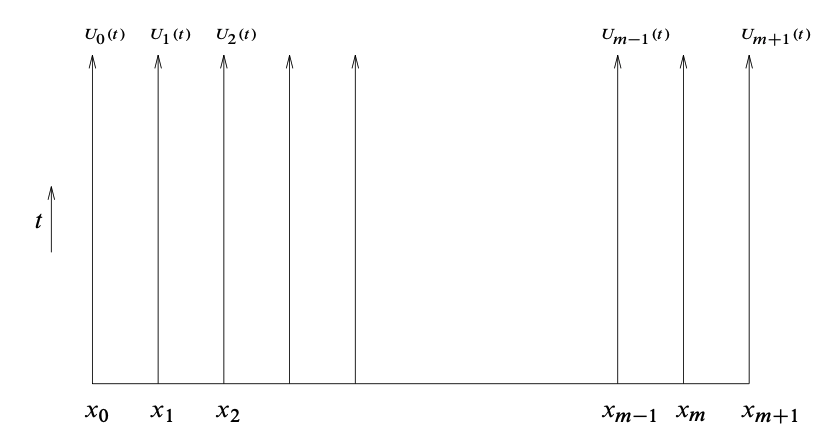
\includegraphics[width=0.95\textwidth]{figures/mol.png} % include the image
    \caption{Method of lines interpretation. $U_i(t)$ is the solution along the line forward in time at the grid point $x_i$ \cite{leveque_fdm}.} 
    \label{fig:mol} % add a label for reference
\end{figure}

Once system of semi-discrete ODE's has been obtained from the MOL, we can apply our chosen time stepping scheme to obtain fully discrete method in which we can isolate the amplifying or dampening factor that affects stability. For ODE absolute stability, this factor is a scalar value (see \textit{Absolute Stability} example below). However, once the MOL has been applied to a PDE, we obtain a system of equations that can be represented as matrices and vectors (if linear). This means the amplifying/dampening factor can be described by analyzing eigenvalues of matrices.

The following provides explicit examples for \textit{Absolute stability}, \textit{Stability Analysis of FTCS} and \textit{Stability analysis of Crank-Nicolson}. 

\vspace{0.5cm}
\begin{tcolorbox}[colback=yellow!5!white,colframe=yellow!75!black]
    \textit{Example: Absolute stability of Forward Euler}

    The notion of \textit{absolute stability} states that an ordinary differential equation (ODE) is absolutely stable under a numerical method if the numerical solution remains bounded as the step size or time step approaches zero, regardless of initial conditions. Consider the following classic ODE: 

    \begin{equation}
        u_t = \lambda u(t) + g(t), \quad u(t_0) = \eta
    \end{equation}

    and its discretization using Forward Euler time stepping

    \begin{equation}
        U^{n+1} = (1 + k\lambda) U^n + k g(t)
    \end{equation}

    where the error

    \begin{equation}
        k\tau^n = u(t_{n+1}) - u(t_n) - k\big(\lambda u(t_n) + g(t_n)\big)
    \end{equation}

    and its LTE:

    \begin{equation}
        \tau^n = \frac{1}{2} k u_{tt}(t_n) + \mathcal{O}(k^2). 
    \end{equation}

    To obtain the global error, subtract the following: 

    \begin{align}
        u(t_{n+1}) &= (1+k\lambda) u(t_n) + k g(t_n) + k \tau^n \\
        U^{n+1}   &= (1+k\lambda) U^{n}  + k g(t_n)
    \end{align}

    to get 

    \begin{equation}
        E^{n+1} = (1+k\lambda) E^n - k\tau^n. 
    \end{equation}

    As the numerical method marches in time, the error is recursively scaled by $(1+k\lambda)$. For $N+1$ total time steps, the final global error is: 

    \begin{equation}
        E^{N+1} = (1+k\lambda)^N E^{N} - k \tau^N.
    \end{equation}
    
    where the superscript $N$ above $E$ represents the second to last time step and the superscript $N$ above $(1+k\lambda)$ obnoxiously represents a power. We expect the to see an exponential grown factor any $k$ for which $|1+\lambda k| > 1$. Therefore we require $|1+k\lambda| \leq 1$ for the Forward Euler method to be absolutely stable. More generally, since $\lambda$ maybe complex, the region of absolute stability is a disk of radius 1, centered at the point -1 (see \Cref{fig:stability}). 

    
\end{tcolorbox}

\vspace{0.5cm}
\begin{tcolorbox}[colback=yellow!5!white,colframe=yellow!75!black]
    \textit{Example: Absolute stability of Trapezoidal}

    Once again, consider the following classic ODE: 

    \begin{equation}
        u_t = \lambda u(t) + g(t), \quad u(t_0) = \eta
    \end{equation}

    and its discretization using Trapezoidal time stepping

    \begin{equation}
        U^{n+1} = U^n + \frac{k}{2}\big(\lambda U^n +  g(t)\big) + \frac{k}{2}\big(\lambda U^{n+1} + g(t_{n+1})\big)
    \end{equation}

    and solving for $U^{n+1}$ and inserting exact solution yields:
    
    \begin{align}
        U^{n+1} &= \frac{(1+\frac{k\lambda}{2})}{(1-\frac{k\lambda}{2})} U^n + \frac{\frac{k}{2}(g^n + g^{n+1})}{(1-\frac{k\lambda}{2})} \\
        U(t_{n+1}) &= \frac{(1+\frac{k\lambda}{2})}{(1-\frac{k\lambda}{2})} U(t_{n}) + \frac{\frac{k}{2}(g^n + g^{n+1})}{(1-\frac{k\lambda}{2})} + k\tau^n. 
    \end{align}

    Subtracting the two and analyzing for the global error: 

    \begin{equation}
        E^{N+1} = \rho^N E^N - k\tau^N, \quad \textit{where } \rho = \frac{(1+\frac{k\lambda}{2})}{(1-\frac{k\lambda}{2})}.
    \end{equation}

    where the superscript $N$ above $E$ represents the second to last time step and the superscript $N$ above $\rho$ obnoxiously represents a power. For absolute stability, we require $|\rho| < 1$. By induction, it is simple to see that $|\rho| < 1 \ \forall \ \lambda k < 0$. This means that the trapezoidal method's stability region is the entire left-hand plane in \Cref{fig:stability}. 

    

    
\end{tcolorbox}

\vspace{0.5cm}
\begin{tcolorbox}[colback=yellow!5!white,colframe=yellow!75!black]
    \textit{Example: Stability analysis of FTCS}
    \vspace{0.25cm}

    As with the analysis of \textit{absolute stability} for an ODE, analysis can be performed on the FTCS method by using first spatially discretizing in space using \textit{Method of Lines} (MOL) to obtain a system of ODEs to interpret the method as a time integration methods of ODEs. 

    For the simple heat equation $u_t = u_{xx}, \ u(t=0) = u_0$, the MOL for FTCS yields a semi-discrete ODE: 

    \begin{equation}
        u_t = \frac{1}{h^2}(U_{m-1}^{n} - 2U_{m}^{n} + U_{m+1}^n), \quad m = 1, \dots, M. 
    \end{equation}

    After temporally discretizing, the boundary conditions can be explicitly encoded in the matrix form: 

    \begin{equation}
        \boldsymbol{U}^{n+1} = (\boldsymbol{I} + k\boldsymbol{A}) \boldsymbol{U}^{n} + k\boldsymbol{g}
    \end{equation}

    where 

    \begin{equation}
        \boldsymbol{A} = 
        \frac{1}{h^2}
        \begin{bmatrix}
            -2 &  1     &        &        &     &    &   \\
            1  & -2     & 1      &        &     &    &   \\
               & \ddots & \ddots & \ddots &     &    &   \\ 
               &        &        &        &  1  & -2 & 1 \\
               &        &        &        &     &  1 & -2
        \end{bmatrix}, \quad 
        \boldsymbol{g} = \frac{1}{h^2}
        \begin{bmatrix}
            g_0(t) = U_0(t) \\
            0 \\
            \vdots \\
            0 \\
            g_{1}(t) = U_{M}(t)
        \end{bmatrix}. 
    \end{equation}

    As in the \textit{absolute stability} example, we can compute the final global error: 
    
    \begin{equation}
        \boldsymbol{E}^{N+1} = (\boldsymbol{I} + k \boldsymbol{A})^N \boldsymbol{E}^N - k \boldsymbol{\tau}^N
    \end{equation}

    where the superscript $N$ above $\boldsymbol{E}$ represents the second to last time step and the superscript $N$ above $(\boldsymbol{I} + k \boldsymbol{A})$ obnoxiously represents a power. More importantly than the inconsistent notation are the eigenvalues of $\boldsymbol{A}$ which determine whether the global error converges or diverges. For the FTCS method to be stable, we require that $k \lambda_m \in \mathcal{S}$.

    For this simple heat equation, the eigenvalues of $\boldsymbol{A}$ are: 

    \begin{equation}
        \lambda_m = \frac{2}{h^2} \big(\cos(m\pi h) - 1\big),\quad \forall m = 1, \dots, M. 
    \end{equation}

    where $h = \frac{1}{m+1}$. The magnitude of $|\lambda_m|$ is largest when $m = M$ and resulting in the eigenvalue: 
    
    \begin{equation}
        \lambda_M \approx \frac{2}{h^2}\big(cos(M \pi h) - 1\big) = \frac{-4}{h^2}.  
    \end{equation}

    Therefore we require that $-k\frac{4}{h^2} \in \mathcal{S}$, which for Forward Euler corresponds to $-2 \leq -k\frac{4}{h^2} \leq 0$, or $\frac{k}{h^2} \leq \frac{1}{2}$.
    
\end{tcolorbox}

\vspace{0.5cm}
\begin{tcolorbox}[colback=yellow!5!white,colframe=yellow!75!black]
    \textit{Example: Stability analysis of Crank-Nicolson}
    \vspace{0.25cm}

    As with the analysis of \textit{absolute stability} for an ODE, analysis can be performed on the FTCS method by using first spatially discretizing in space using \textit{Method of Lines} (MOL) to obtain a system of ODEs to interpret the method as a time integration methods of ODEs. 

    For the simple heat equation $u_t = u_{xx}, \ u(t=0) = u_0$, the MOL for FTCS yields a semi-discrete ODE: 

    \begin{equation}
        u_t = \frac{1}{h^2}(U_{m-1}^{n} - 2U_{m}^{n} + U_{m+1}^n), \quad m = 1, \dots, M. 
    \end{equation}

    
\end{tcolorbox}

% Recall the \textit{Crank-Nicholson for linear PDEs} example in which \cref{eq:heat_simple} was discretized in space using MOL, and then in time using the trapezoidal method. 

% An alternative (and simpler) method to analyzing the stability of the Crank-Nicolson method for \cref{eq:heat_simple} is to use the \textit{Von Neumann} approach. This analysis involves making an ansatz (assumption) that the numerical solution has a certain form, and then deriving a condition on the time step that ensures that the numerical solution does not grow without bound.

% First, assume that the numerical solution has the form:

% \begin{equation}
%     u_m^n = e^{i\omega mh} \phi^n, 
% \end{equation}

% where $h$ is the spatial step size, $k$ is the time step size, $\omega$ is the wave number, $m$ is the spatial index, and $n$ is the time index. Substituting this form into the Crank-Nicolson method and solving for $\phi^{n+1}$, we obtain:

% \begin{equation}
%     \phi^{n+1} = \frac{1+\frac{\theta}{2}i\omega h^2}{1-\frac{\theta}{2}i\omega h^2} \phi^n
% \end{equation}

% where $\theta$ is a parameter that controls the weighting between the backward and forward differences in time, and is given by $\theta = \frac{k}{h^2}$.

% The von Neumann stability analysis requires that the amplification factor $G(\omega,k) = \frac{\phi^{n+1}}{\phi^n}$ satisfies $|G(\omega,k)| \leq 1$ for all $\omega$ and $k$, in order to ensure that the numerical solution does not grow without bound.

% Solving for the absolute value of the amplification factor, we obtain:

% \begin{equation}
%     |G(\omega, k)| = \bigg| \frac{1 + \frac{\theta}{2} i \omega h^2}{1 - \frac{\theta}{2} i \omega h^2}\bigg|, 
% \end{equation}

% which simplifies to:

% \begin{equation}
%     |G(\omega, k)| = \frac{1 + \frac{1}{2}\theta(\omega h)^2}{1 - \frac{1}{2}\theta(\omega h)^2}. 
% \end{equation}

% To ensure that $|G(\omega,k)| \leq 1$ for all $\omega$ and $k$, we require that $\theta \leq 1$. This condition is the stability criterion for the Crank-Nicolson method for the heat equation, and it ensures that the numerical solution does not grow without bound, regardless of the time step size.

\begin{figure}[h]
  \centering
  \begin{minipage}[b]{0.3\linewidth}
    \centering
    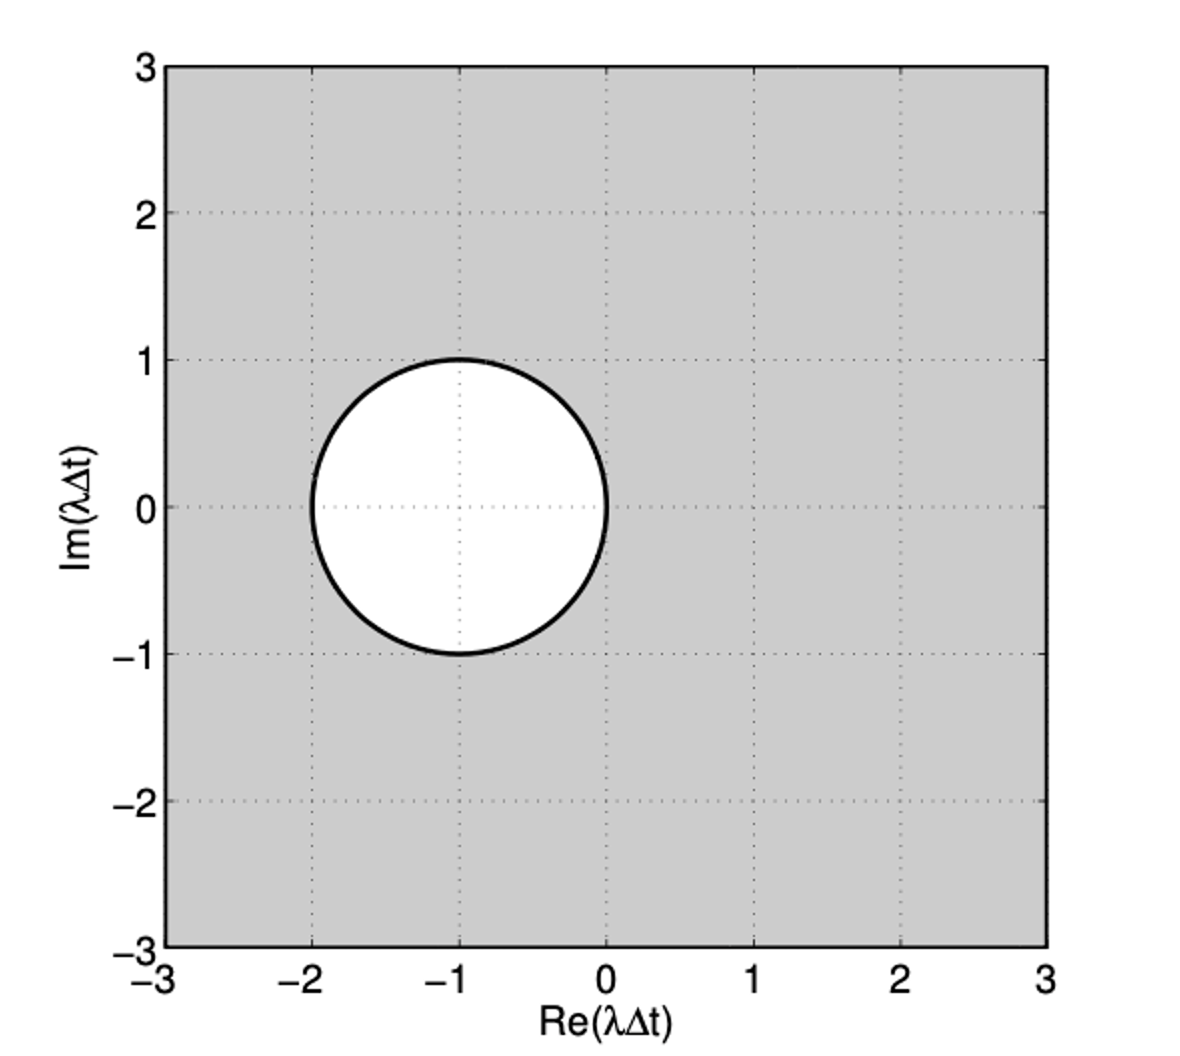
\includegraphics[width=\linewidth]{figures/fe_stability.png}
  \end{minipage}
  \hspace{0.01\linewidth}
  \begin{minipage}[b]{0.3\linewidth}
    \centering
    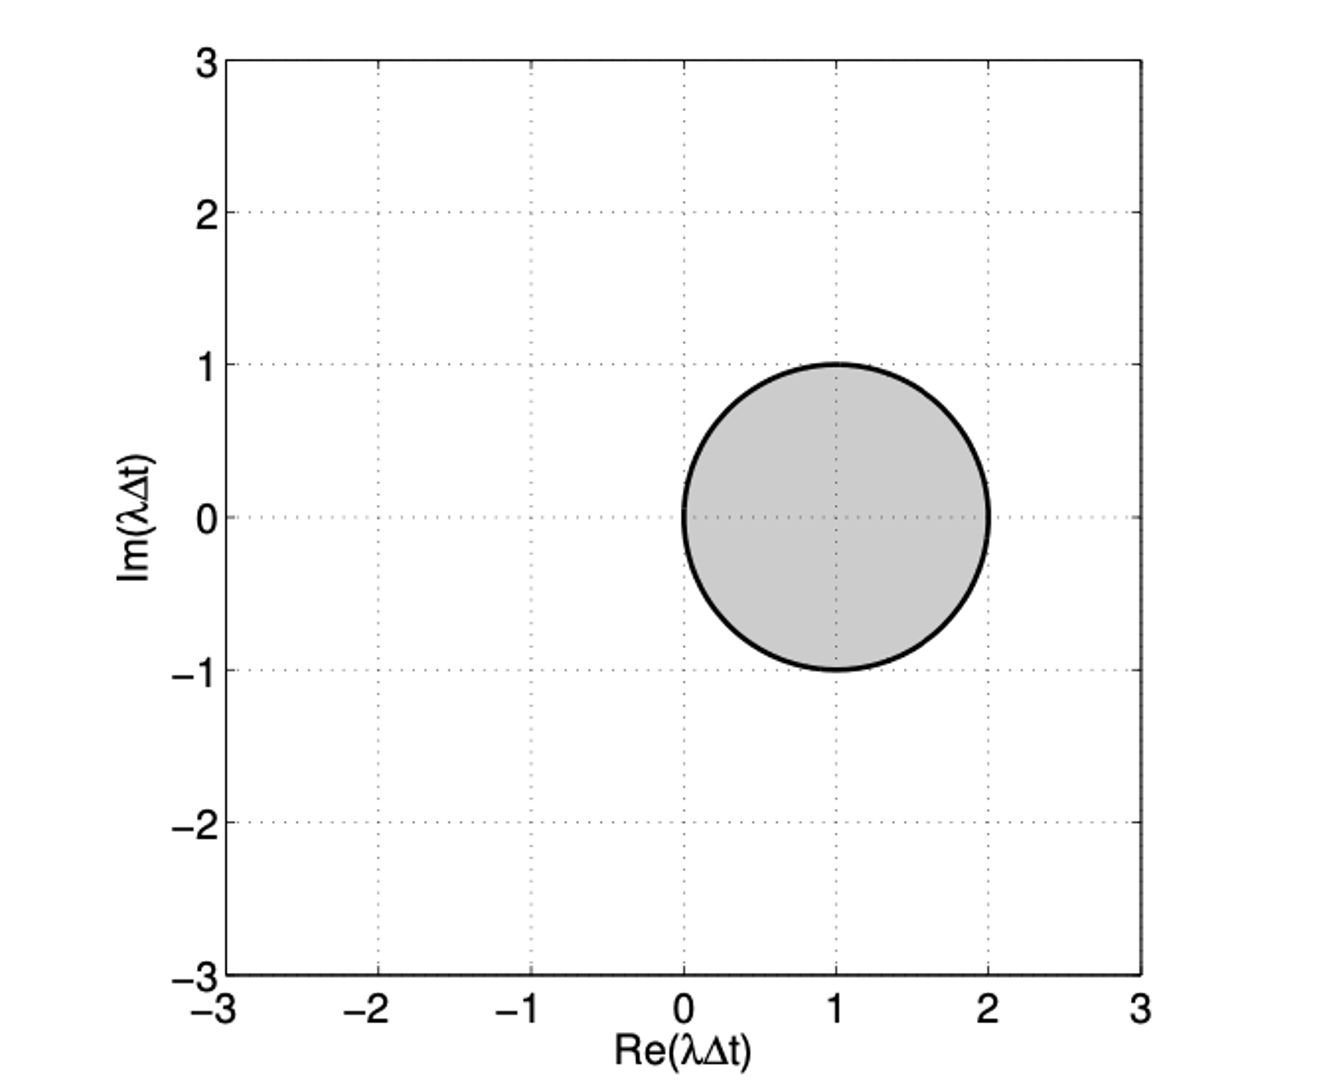
\includegraphics[width=\linewidth]{figures/be_stability.png}
  \end{minipage}
  \hspace{0.01\linewidth}
  \begin{minipage}[b]{0.3\linewidth}
    \centering
    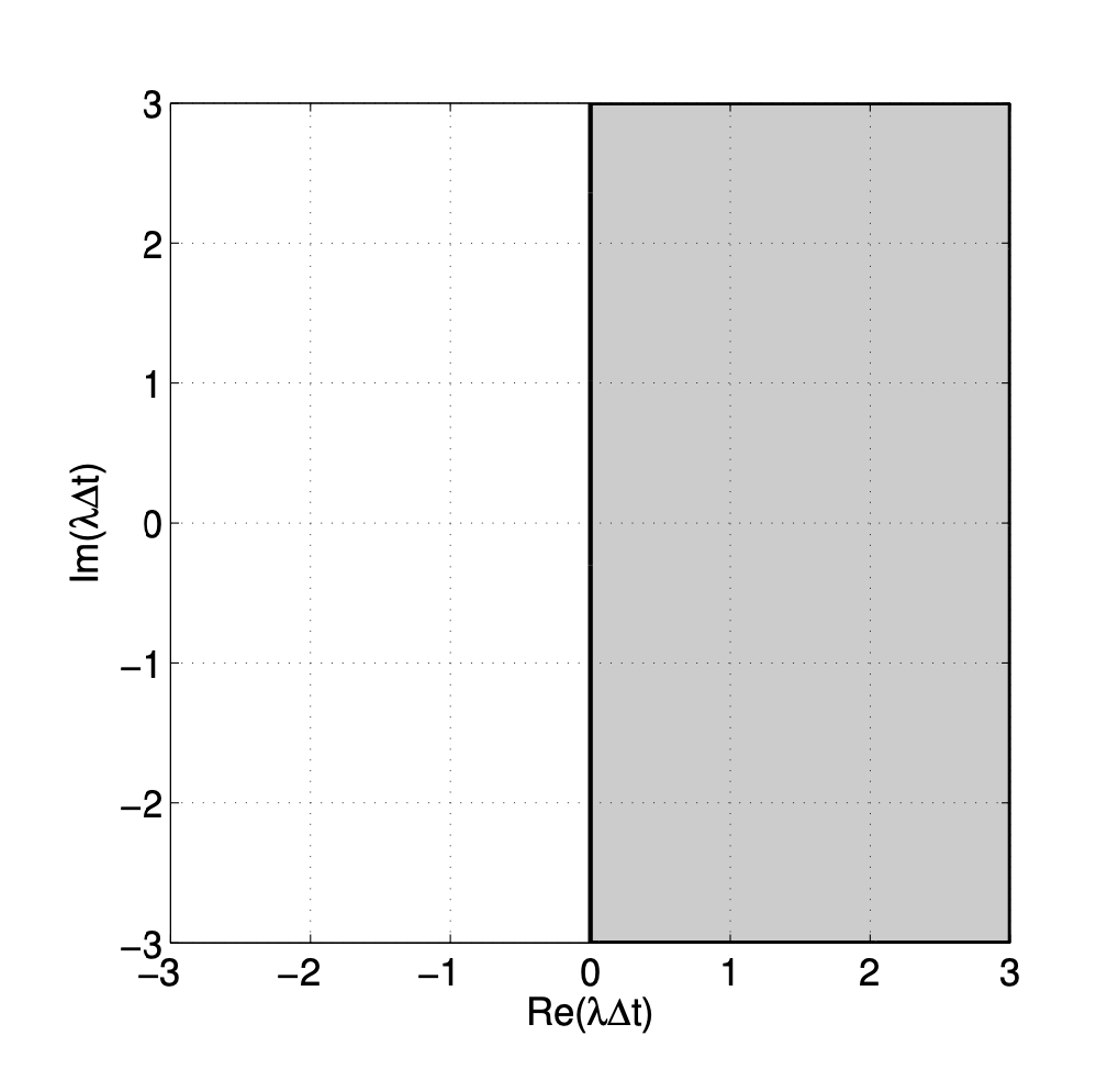
\includegraphics[width=\linewidth]{figures/trap_stability.png}
  \end{minipage}
  \caption{A comparison of the stability regions for 1) Forward Euler, 2) Backward Euler and 3) Trapezoidal where the white area corresponds to stability (the absolute stability region) and the gray area to instability \cite{num_methods_mit}}
  \label{fig:stability}
\end{figure}


\vspace{0.5cm}
\noindent\textbf{Convergence}

The Dahlquist Equivalence Theorem is the primary tool for assessing whether or not a numerical scheme is convergent. Using the concepts of consistency and zero stability alone, we can draw a conclusion about the convergence. To summarize from above, we have the following concepts:

\begin{itemize}
    \item Consistency: \quad In the limit $k \rightarrow 0$, the method gives a consistent discretization of the ordinary differential equation. 
    \item Zero stability: \quad In the limit $k \rightarrow 0$, the method has now solutions that grow unbounded as $N = T / k \rightarrow \infty$. 
\end{itemize}

The Dahlquist Equivalence Theorem guarantees that a method is consistent and stable is convergent, and also that convergent method is consistent and stable.


